\chapter{Introduction}

Humanoid robots garner much interest not only in the fields of engineering and science, but over a wide range of social and non-technical contexts. The humanoid form makes robots more relatable and accepted by the general public. Socially assistive and service robots need this sort of acceptance in order to perform their jobs more effectively. 
They also offer unique opportunities for robots to operate in environments which are commonly designed for humans. These environments are typically difficult for many robots to operate in due to things such as narrow corridors, varying heights of door knobs and handles, and stairs.
With the ability to traverse a wide range of terrains from rubble to stairs and the dexterity offered by multiple degree-of-freedom manipulators and fingers, humanoids as a platform have a flexibility not seen in many mobile robots. This makes them desirable for operating not only in human structured environments, but unstructured environments such as construction and disaster scenarios.

With such mechanical flexibility come many challenges. Efficient and adaptable gaiting for humanoids is an active and heavily studied area of research, as well as the perception capabilities necessary to take advantage of such robust possible modes of operation. Facial, object, and speech recognition, localization, mapping, path planning, neural and semantic networks are just some of the perception areas researched in order to get humanoids to operate in natural human environments.
Aside from the algorithmic challenges of leveraging humanoid platform capabilities, designing platforms with efficient mechanical and electrical systems to accommodate difficult weight and power requirements make this field rife with interesting and novel research possibilities. Vision, structured light, planar laser scanning, series-elastic actuation, and harmonic drive systems are a few of the sensing and actuation topics particularly applicable to humanoid research.

For this project, the Nao humanoid platform by Aldebaran Robotics was used. Nao is approximately two feet tall, with 25 degrees-of-freedom, and various sensors including HD cameras, ultrasonic distance sensors, and inertial sensors. It is easily programmed with a graphical programming interface called Choreographe, or through a framework called NAOqi in which multiple text-based languages such as C++ and Python can be used. Through either API, prebuilt routines such as gaiting and object tracking can be used, allowing for other areas utilizing such commonly needed tasks to be explored, though custom algorithms can be written to supplement or replace the prebuilt ones.

In this project, the topic of path planning was explored.
The path planning problem consists of moving a mobile platform or end-effector from a start location to a goal location.
Examples vary from ground robots moving through an office building, UAVs navigating to GPS waypoints, or end-effectors avoiding objects on a cluttered table to grasp an object.
Methods of solving such a problem depend largely on the construction and knowledge of the environment and the knowledge the robot has about its position within the environment. For example, a mobile robot operating in the plane within a static environment, \textit{a priori} map, and direct position sensing has different challenges than a mobile robot operating in three-dimensions, within an unknown dynamic environment, and only platform velocity estimation.
Popular approaches include graph search algorithms such as A* or D*, Bug algorithms, and potential fields approaches. Potential fields algorithms treat the mobile robot as a point mass that is repelled by obstacles and attracted by the goal. 

The algorithm implemented was the Game-Theoretic Optimal Deformable Zone with Inertia and Local Approach (GODZILA) algorithm. It is a potential fields style algorithm, with additions that add a form of inertia to reduce limit-cycles and local mimima, a straight-line planner for when the goal is insight, and a goal-randomizer for when the robot is stuck. The ultrasonic sensors on the Nao were used to estimate distance to obstacles, while the prebuilt red ball tracker routine that uses Nao's HD cameras to estimate range and bearing to a 6 cm diameter red ball was used to indicate the location of the goal. Prebuilt gaiting algorithms were used to command the Nao to linear and angular velocities. This allowed the Nao to walk towards a goal with multiple obstacles interfering in its path.

\begin{comment}

\begin{figure}[h]
	\centering
	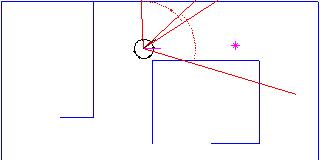
\includegraphics{sim_fig1.jpg}
	\caption[Planar robot simulation example.]
	{Planar robot simulation example. The robot is indicated by a black circle with the red cones simulating ultrasonic sensor beams and their detected range indicated by dotted red arcs in the red cone. Blue lines represent obstacles. The magenta line points towards the goal location, which is indicated by a magenta star.}
	\label{fig:simFig1}
\end{figure}

\end{comment}




